Tunel $ \Tau $ v molekule je v našem případě modelován posloupností koulí o různých poloměrech umístěných v prostoru. Pro posloupnost koulí $ \Tau = \{S_i\}_{i=0}^{n} $ navíc platí $ S_i \bigcap S_{i+1} \neq \emptyset $ pro všechna $ 0 \leq i < n $.
Pro představu jak takový tunel může vypadat uvádíme obrázek \ref{fig:basic_tunnel}.
\begin{figure}[ht]
  	\centering
	\includegraphics[width=100mm]{img/basic_tunnel.jpg}
	\caption{Sample of molecule tunnel}
  \centering
  \label{fig:basic_tunnel}
\end{figure}


Abychom mohli provádět docking ligandu, musíme nejprve takto definovaný tunel nařezat na jemné plátky - kruhy, na které pak v průběhu výpočtu budeme dokovat průběžné konformace ligandu. Popišme si nyní, jak by takové řezy měly vypadat.

\begin{defi}
Řezem tunelu $ \Tau $ rozumíme kruh v prostoru, který je určen uspořádanou trojicí $\theta = (A, u, r)$, kde $ A $ je střed, $ u \in \Rbb^3 $ je normálnový vektor a $ r > 0 $ je poloměr.
Pro tento kruh $ \theta $ musí platit, že $ \Tau \cap \theta $ je souvislá množina a navíc
$ \exists \delta > 0 $ tak, že $ \forall \varepsilon > 0,  \varepsilon < \delta $ je  $ (A, u, r + \varepsilon) \cap \Tau = \theta \cap \Tau $.
(Alternativně řečeno $\Tau \setminus \theta $ má dvě komponenty.)
\end{defi}

Uvedená definice prakticky říká, že řez tunel řeže jen na jednom místě (podmínka souvislosti). Druhá podmínka znamená, že řez je úplný, tedy že řezem skutečně rozdělíme tunel na dvě části.
Pro ilustraci, jak takové řezy mohou vypadat, přikládáme obrázek č. \ref{fig:tunnel_cuts}.
\begin{figure}[ht]
    \centering
    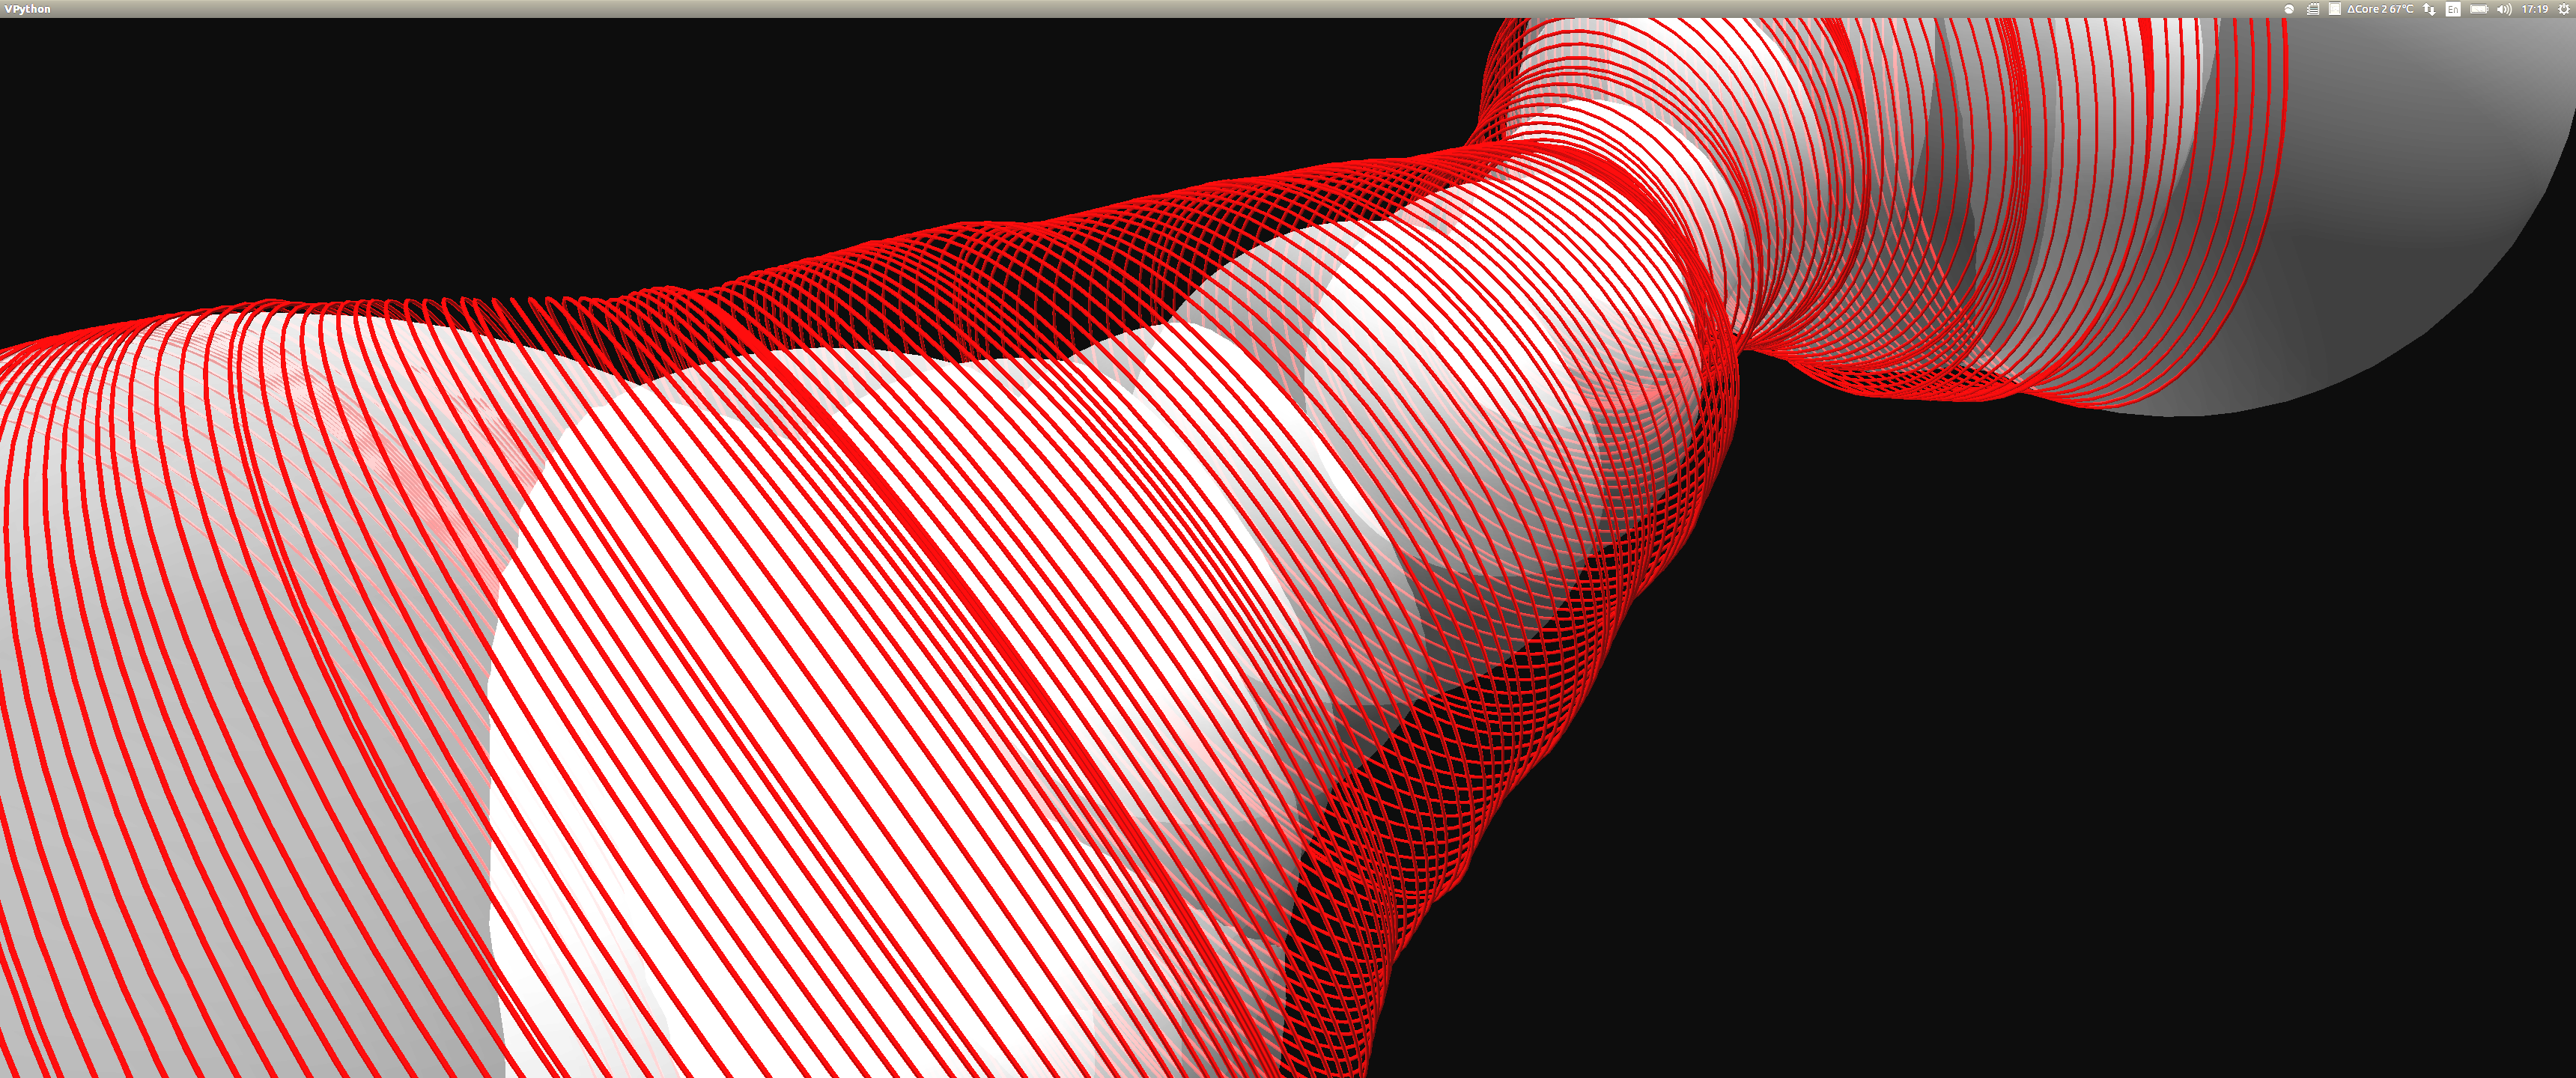
\includegraphics[width=\textwidth]{img/simple_cuts.png}
    \caption{Sample of molecule tunnel}
  \centering
  \label{fig:tunnel_cuts}
\end{figure}

S takto definovanými řezy můžeme začít uvažovat o tom, jak tunel nařezat jako celek.
Mějme $ \Theta = \{\theta_i\}_{i=0}^{k}$ posloupnost řezů tunelu $ \Tau $. Pro potřeby správného
dockingu bude nezbytné, aby platilo $ x, y \in \Theta \Rightarrow |x \cap y| \leq 1 $,
tedy každé dva řezy se dotýkají nejvýše v jednom bodě. Dále budeme chtít, aby po sobě
jdoucí řezy od sebe \textit{nebyly příliš daleko}. Vzdálenost budeme měřit pomocí funkce
$ \dst(x, y) $, kterou popisuje následující definice.

\begin{defi}
Mějme řezy $ x = (A, u, r_1), y = (B, v, r_2) \in \Theta $. Rozlišíme dvě situace
    \begin{enumerate}[label={(\arabic*)}]
        \item $ u = v $, pak vezmeme libovolný vektor $ w $ tak, aby
            $ \varrho = \langle u, w \rangle $ tvořilo rovinu.
        \item V opačném případě položíme přímo $ \varrho = \langle u, v \rangle $.
    \end{enumerate}
Kolmou projecí do roviny $ \varrho $ promítneme řezy $x $ resp. $y$, čímž získáme dvě úsečky
určené vrcholy $X_1, X_2 $ resp $Y_1, Y_2 $. Vzdálenost pak definujeme jako
    \begin{center}
        $ \dst(x, y) = \min\{ \max\{|X_1 - Y_1|, |X_2 - Y_2|\}, \max\{|X_1 - Y_2|, |X_2 - Y_1|\}\}$.
    \end{center}
\end{defi}

Nyní můžeme přistoupit k popisu samotného algoritmu, který má na vstupu tunel $ \Tau $
a nějaké pevně zadané $ \delta > 0$, které určuje maximální vzdálenost, kterou
od sebe dva po sobě jdoucí řezy mohou mít. Na výstupu pak budeme očkávat řezy pokrývající
celý tunel a budou splňovat uvedené omezení na vzdálenost. Vzhledem k tomu, že výsledná
složitost následného dockingu je přímo úměrná počtu řezů, budeme od algoritmu také chtít,
aby počet řezů byl při splnění uvedených kritérií pokud možno co nejmenší.


\subsection{Algoritmus}

Celý algoritmus se sestává z celé řady funkcí řešících méně či více důležité podproblémy.
Domníváme se, že vyčerpávající popis všech komponent by byl zbytečně technický a snad i
ubíjející, proto se zde zaměříme zejména na popis těch opravdu klíčových, zajímavých
a tam, kde implementace nějakého výpočtu nebude důležitá pro pochopení fungování
algoritmu jako celku, se omezíme pouze na symbolický zápis, případně stručný slovní
popis.

Pro začátek si řekněme něco o základní kostře algoritmu. Přirozeným naivním přístupem
k řešení našeho problému, by bylo vzít trajektorii tunelu tvořenou středy koulí
jím definované, po této trajektorii se s krokem $ \delta $ posouvat a generovat
řezy se středem na trajektorii a normálou určenou směrem pohybu na trajektorii.
Takovýto přístup by fungoval vcelku dobře pro tunely, které by byly relativně
přímé bez zatáček, avšak pro \say{klikaté} tunely by generoval řezy zcela nepoužitelné.
Pro ilustraci uvádíme obrázek \ref{fig:naive_cuts}.

\begin{figure}[ht]
    \centering
    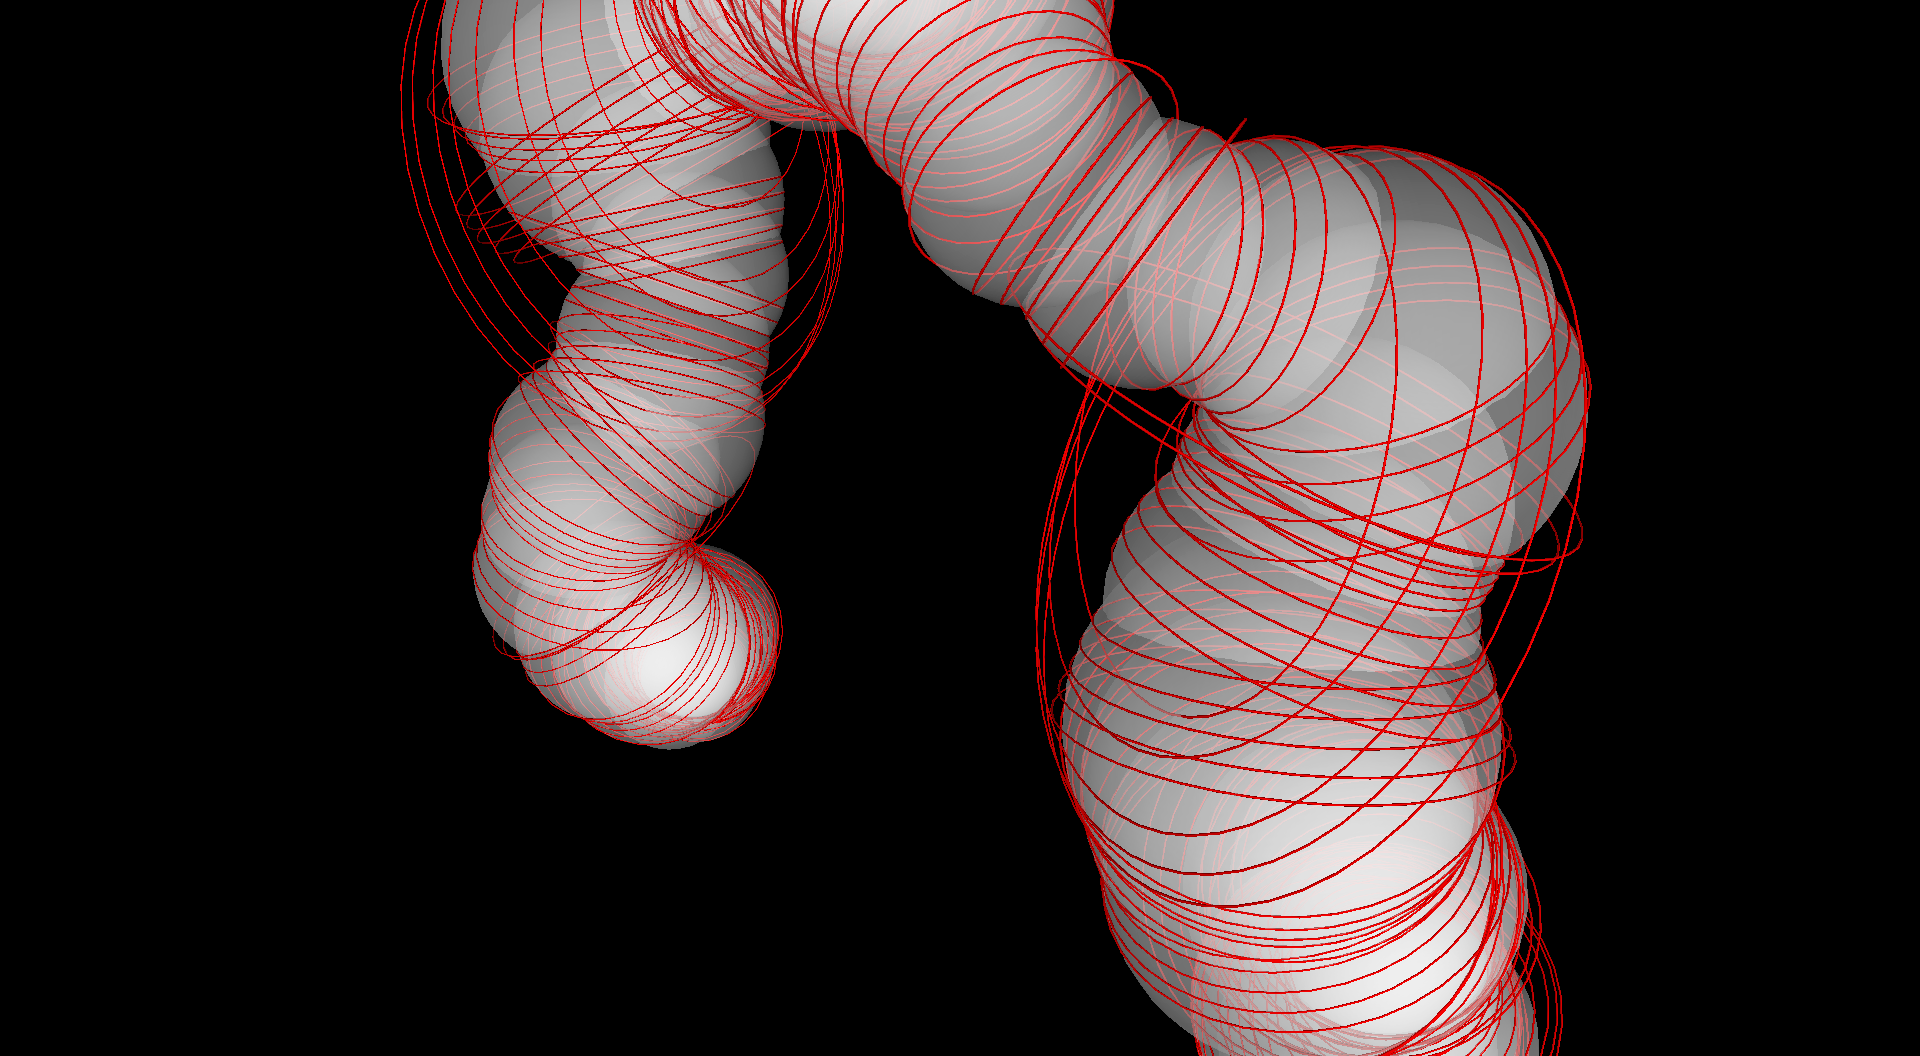
\includegraphics[width=\textwidth]{img/naive_cuts.png}
    \caption{Naive cuts}
  \centering
  \label{fig:naive_cuts}
\end{figure}

K problémům docházi proto, že bere v potaz pouze velmi lokální informace o vlastnostech
tunelu a zřejmě zcela ignorujeme dříve uvedené požadavky na řezy. Tento postup ale
můžeme zdokonalit. Prvním problémem je, že když takto postupně generujeme nové řezy,
může se stát, že od sebe budou příliš daleko nebo se budou protínat. Potřebujeme proto
funkci $ shiftNewDisk $, která přesně toto zajistí. Jak ale můžeme vidět na obrázku
\ref{fig:shift_cuts}, toto způsobí, že se v případě nevhodné orientace normálových
vektorů sice zachovají naše požadavky na řezy, avšak dostaneme jich zbytečně mnoho.

\begin{figure}[ht]
    \centering
    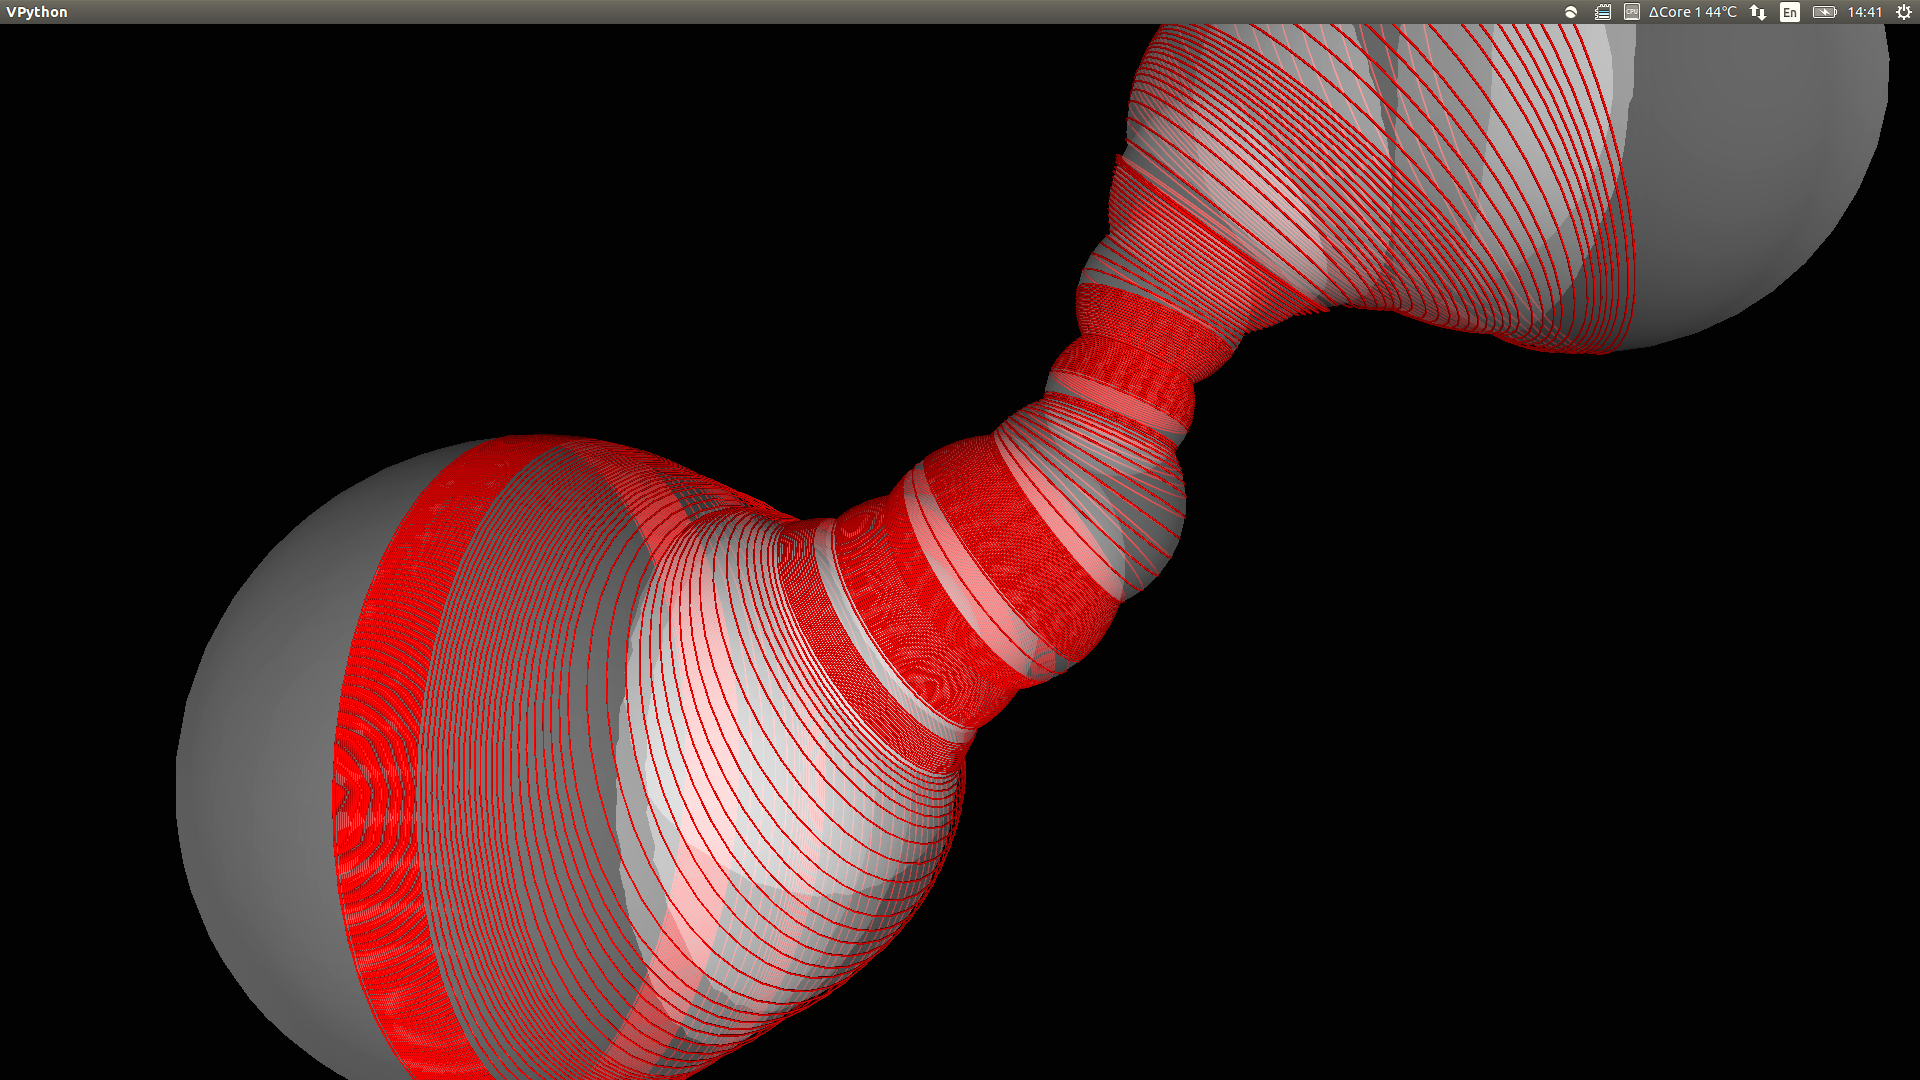
\includegraphics[width=\textwidth]{img/shift_cuts.png}
    \caption{Shifting cuts}
  \centering
  \label{fig:shift_cuts}
\end{figure}

Z toho důvodu je ještě vhodné po každém posunu zkontrolovat, zda nemůžeme předchozí
řez prostě jen nahradit novým řezem $ \theta $. To jest pro
$ \theta_{i - 2} \in \Theta $ zkontrolovat zda náhodou neplatí
$ \dst(\theta_{i - 2}, \theta) < \delta $. Pokud ano, můžeme zřejmě nahradit
$ \theta_{i - 1} = \theta $. (Toto má samozřejmě smysl jen pokud
$ |\Theta| > 1 $.) Jak můžeme vidět na obrázku \ref{fig:cuts_with_replace}
výsledek již vypadá o mnoho lépe.

\begin{figure}[ht]
    \centering
    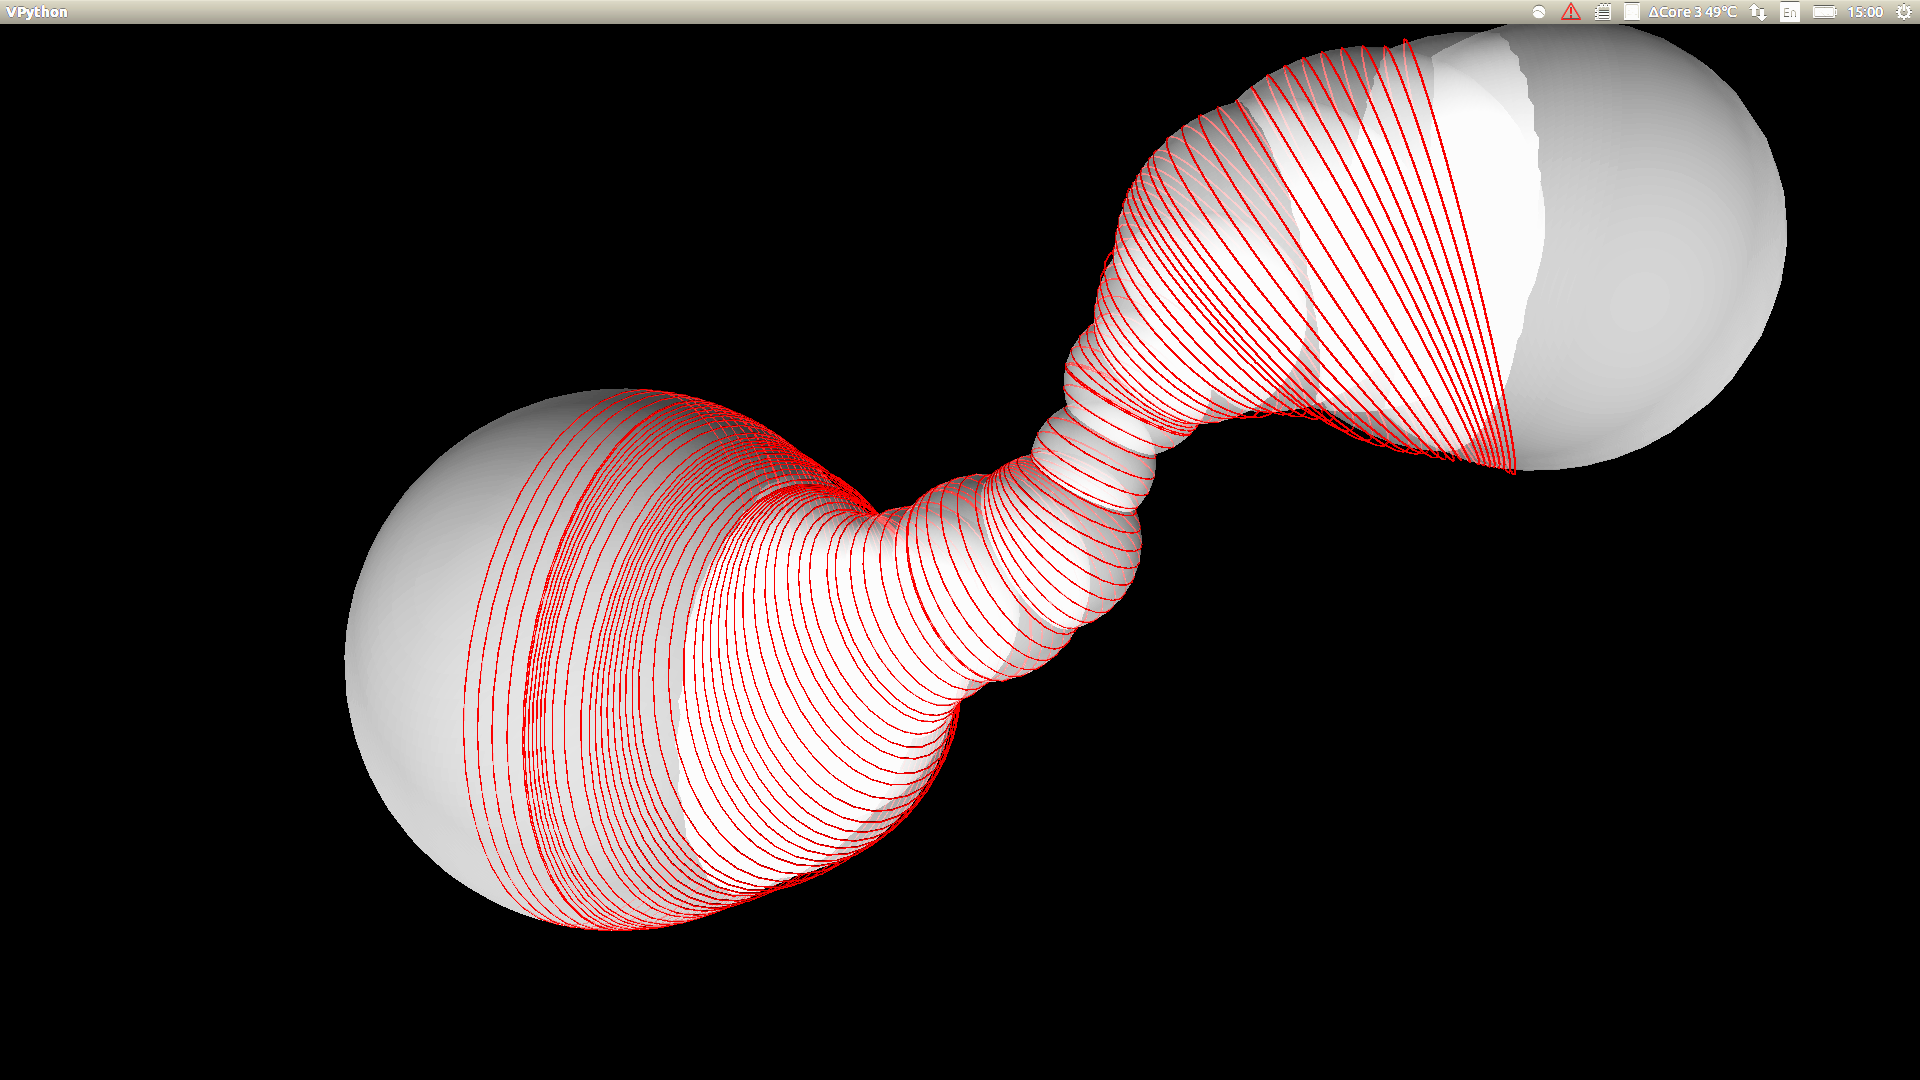
\includegraphics[width=\textwidth]{img/cuts_with_replace.png}
    \caption{Cuts with replace}
  \centering
  \label{fig:cuts_with_replace}
\end{figure}

Jak si ale pozorný čtenář může povšimnout, na pravém konci tunelu uvedeného na
posledním obrázku můžeme vidět, že řezy nezatáčí tak jak by mohly a nekopírují tak
profil tunelu příliš věrně. Po krátkém zamyšlení se dá nahlédnout, že tomu tak
je pravděpodobně kvůli tomu, jaké volíme výchozí normálové vektory pro jednotlivé
řezy. Pokud řezy orientujeme výhradně podle lokálních vlastností trajektorie,
tak se nám může stát, že právě například nezačneme zatáčet dostatečně brzy apod.
Z tohoto důvodu budeme pro výpočet normály nového řezu používat třídu
$ TunnelCurve $ a její metodu $ getWeightedDir $, která pro daný bod $ P $ na křivce
- trajektorii tunelu spočítá vážený průměr směrových vektorů této křivky na
okolí bodu $ P $. Exaktněji tento výpočet a případná zlepšení rozvedeme později.
Pro ilustraci se ještě podívejme na obrázek \ref{fig:weighted_dir}. Je vidět, že
řezy nyní kopírují zakřivení tunelu mnohem ochotněji.

\begin{figure}[ht]
    \centering
    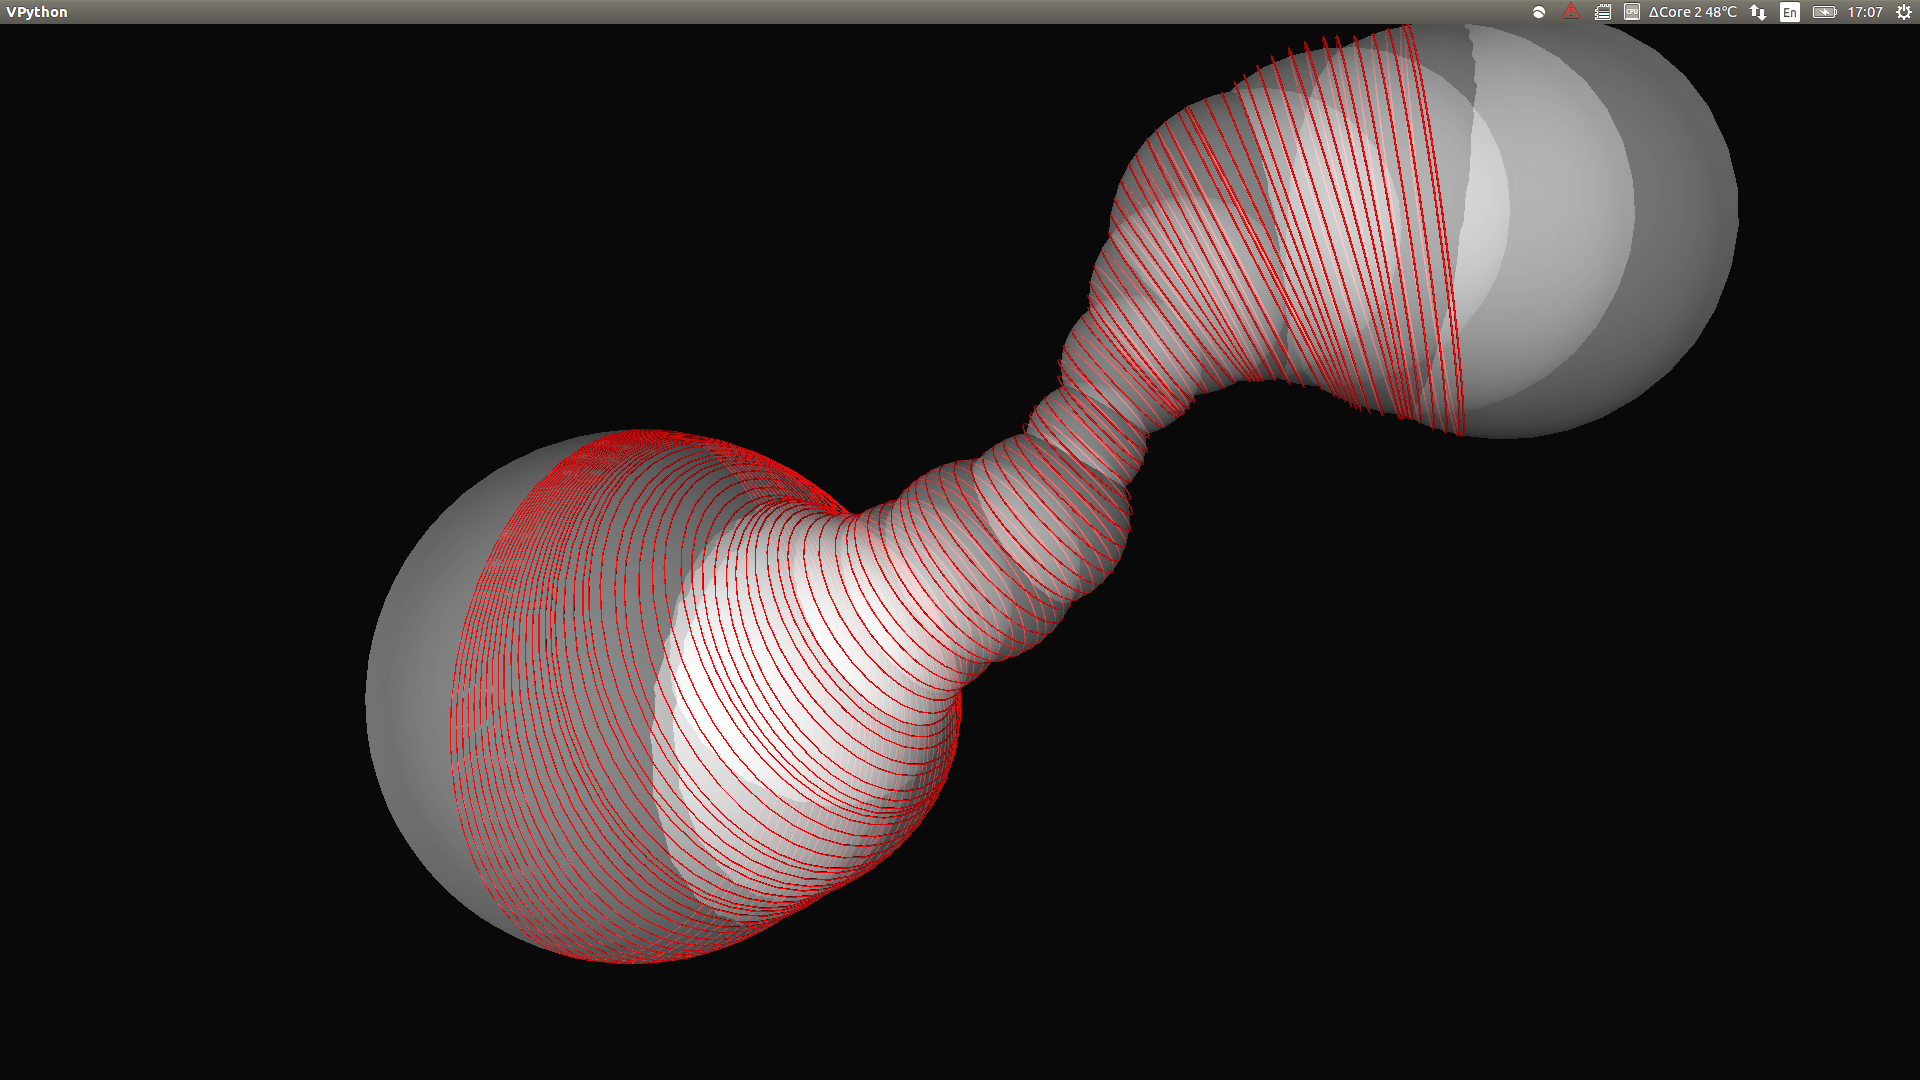
\includegraphics[width=\textwidth]{img/weighted_dir.png}
    \caption{Cuts with weighted direction}
  \centering
  \label{fig:weighted_dir}
\end{figure}

Kostru naznačeného algoritmu zachycuje následující pseudokód.

\begin{algorithm}
\begin{algorithmic}

\Function{digTunnel}{$\Tau, \delta$}
    \State $ centers \gets [ S_{center} \in \Tau ] $
    \State $ normals \gets [ \operatorname{norm}(C_{i + 1} - C_{i}) \mid 0 \leq i < |centers| ] $
    \State $ disks \gets   [fitDiskTunnel(normals[0], centers[0], 0, \Tau, \delta)] $
    \State $ curve \gets \operatorname{TunnelCurve}(centers) $
\EndFunction

\end{algorithmic}
\end{algorithm}


\end{document}
